\documentclass[UTF8]{ctexart}
\usepackage{ctex}
\usepackage{geometry}
\usepackage{enumitem}
\usepackage{indentfirst}
\usepackage{color}
\usepackage{fancyhdr}
\usepackage{amsmath}
\usepackage{graphicx}
\usepackage{amssymb}
\usepackage{tikz}
\usepackage{cases}
\usepackage{array}
\usepackage{pgfplots}
\usepackage{tkz-euclide}
\usepackage{mathrsfs}
% 设置纸张和页边距——A4
\geometry{papersize={21cm,29.7cm}}
\geometry{left=3.18cm,right=3.18cm,top=2.54cm,bottom=2.54cm}

% 一级标题靠左
\CTEXsetup[format={\Large\bfseries}]{section}

% 去除页眉
\pagestyle{plain}

%设置段间距
\addtolength{\parskip}{.4em}
%%设置行间距
%\usepackage{setspace}
%\setstretch{2.5}

% 开始文档内容
\begin{document}

\title{信号与系统课程笔记:Lecture 22\par
零极图,系统函数H(s)}
\author{授课教师:秦雨潇 \\
        笔记记录:曹时成}
\date{2023 年 11 月 24 日(第十二周,周五)}
\maketitle

\section{复习}
\subsection{拉普拉斯变换}
$y''(t) + ay'(t) + by(t) = cf(t)$ \qquad $ \longleftrightarrow $ \qquad $ h(t)=k_1e^{-p_1t}+k_2e^{-p_2t}$ \par
\qquad \qquad $\updownarrow s \text{域}$ \qquad \qquad \qquad \qquad \qquad \qquad \qquad \qquad $\updownarrow \mathscr{L}$ \par
$s^2Y(s)+asY(s)+bY(s)=cF(s)\longleftrightarrow H(s)=\frac{Y(s)}{F(s)}=\frac{c}{s^2+as+b}= \frac{k_{1}}{(s-p_1)}+\frac{k_{2}}{(s-p_2)} $ \par
\subsection{零极图}
\begin{figure}[h]
    \centering         %使图片居中放置
    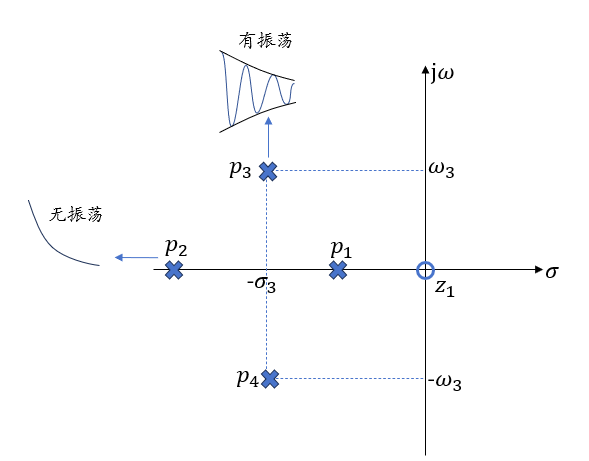
\includegraphics[scale=0.45]{1.png}
    \caption{零极图}
\end{figure}
\subsection{零极图的作用}
(1)可以得到H(s)\par
例:$H(s)=\frac{k(s-0)}{\prod _{i=1}^n(s-p_i)} $ \par
(2)零极图可以直接看出系统的“属性”\par
例:$h(t)=k_1e^{-p_1t}+ k_2e^{-p_2t}+k_3e^{-\delta_3t}cosw_3t$ \par

\section{零极图的作用3:设计系统}
第一步:观察一下\par
$H(s)\longleftrightarrow H(w)$ \qquad $e^{jw_0}\ast h(t)=|H(w_0) \vert e^{j(w_0+\angle H(w_0))} $\par
$H(w)=H(s)\vert _{s=jw\text{或}\delta=0}$\par
$| H(w)\vert =| H(s)\vert =|\frac{\prod _{i=1}^m(s-z_i)}{\prod _{i=1}^n(s-p_i)}  \vert =\frac{\prod _{i=1}^m| (s-z_i)\vert}{\prod _{i=1}^n| (s-p_i)\vert }\vert _{s=jw\text{或}\delta=0}$\par
零极图设计系统\par
\begin{figure}[h]
    \centering         %使图片居中放置
    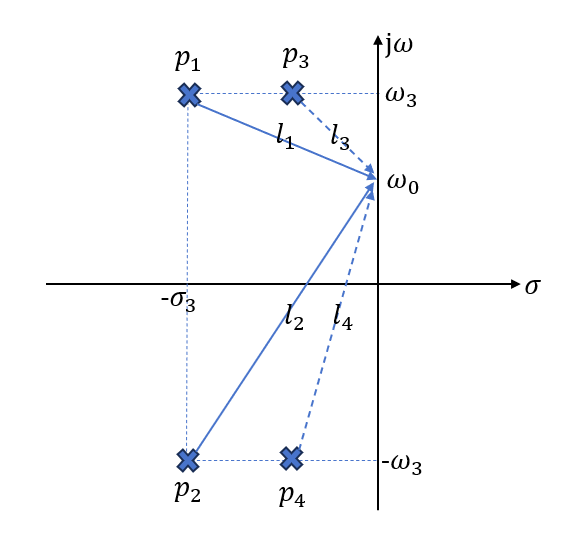
\includegraphics[scale=0.45]{2.png}
    \caption{零极图对应系统的解释}
\end{figure}
$| H(w)\vert =\frac{\prod _{i=1}^m| (s-z_i)\vert}{\prod _{i=1}^n| (s-p_i)\vert }\vert _{s=jw}=\frac{\prod _{i=1}^m| (jw-z_i)\vert}{\prod _{i=1}^n| (jw-p_i)\vert }$\par
$\equiv \frac{|C_{z_1} \vert|C_{z_2} \vert|C_{z_3} \vert }{|C_{p_1} \vert|C_{p_2} \vert|C_{p_3} \vert} $\par
其中$|l_1 \vert=| \overrightarrow{p_1w_0}\vert  =|jw_0-p_1 \vert =|C_{p_1} \vert $\par
当 $| l_1\vert \cdot | l_2\vert $ 最大时,$H(w_0)$最小\par
当 $| l_1\vert \cdot | l_2\vert $ 最小时,$H(w_0)$最大\par
极点靠近jw轴时:$| l_3\vert \cdot | l_4\vert< | l_1\vert \cdot | l_2\vert\Longrightarrow H(w)_{| l_1\vert \cdot | l_2\vert}>H(w)_{| l_3\vert \cdot | l_4\vert}$\par
\subsection{LPF}
\begin{figure}[h]
    \centering         %使图片居中放置
    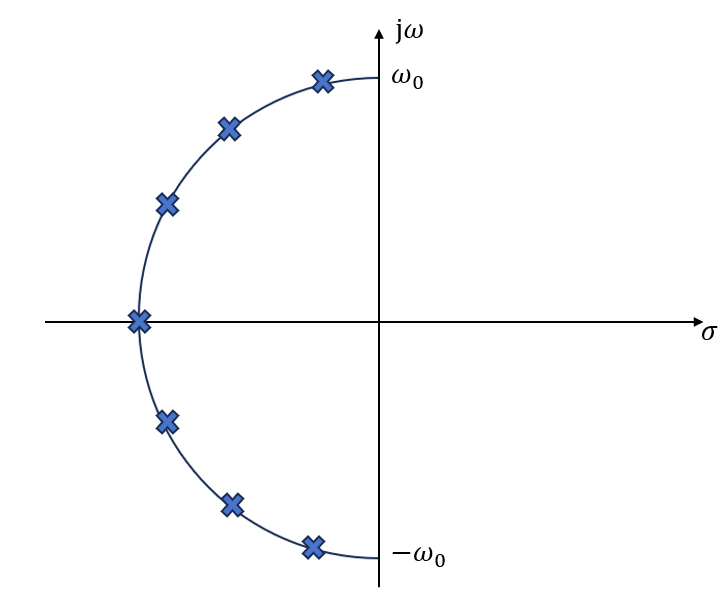
\includegraphics[scale=0.25]{3.png}
    \caption{巴特沃斯滤波器(Butterworth Filter)的零极图}
\end{figure}
极点数越多,滤波器衰减越快,但系统设计难度越大。\par
\subsection{BPF,带通滤波器}
\begin{figure}[h]
    \centering         %使图片居中放置
    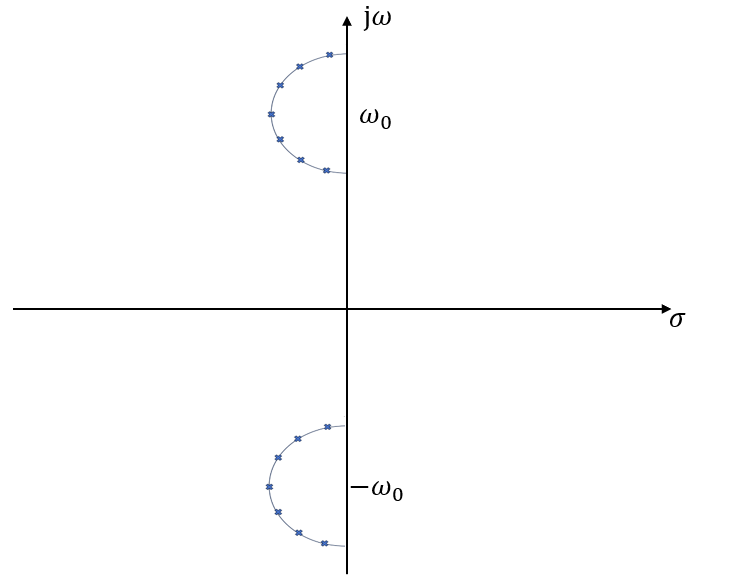
\includegraphics[scale=0.45]{4.png}
    \caption{带通滤波器的零极图}
\end{figure}
\subsection{Notch Filter,带阻滤波器}
\begin{figure}[h]
    \centering         %使图片居中放置
    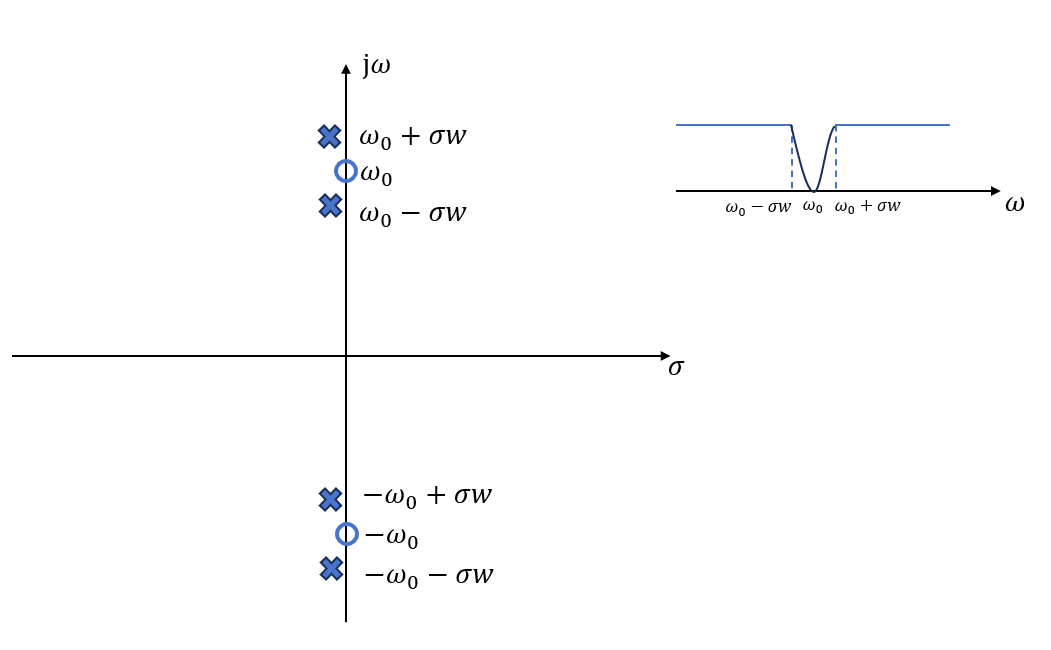
\includegraphics[scale=0.45]{5.png}
    \caption{带阻滤波器的零极图}
\end{figure}
\section{框图}
需求$ \xrightarrow{\text{Z-P图}} $ H(s)$\longrightarrow $ 微分方程$ \xrightarrow{\text{框图}} $ “电路”\par
$y''(t) + ay'(t) + by(t) = cf(t)$ \par
\subsection{框图的基本元素}
(1)基本运算逻辑:加法;乘法;微分。 \par
(2)基本运算单元:“加法器”;:“乘法器”;“积分器”。 \par
(3)基本框图元素:\par
\begin{figure}[h]
    \centering         %使图片居中放置
    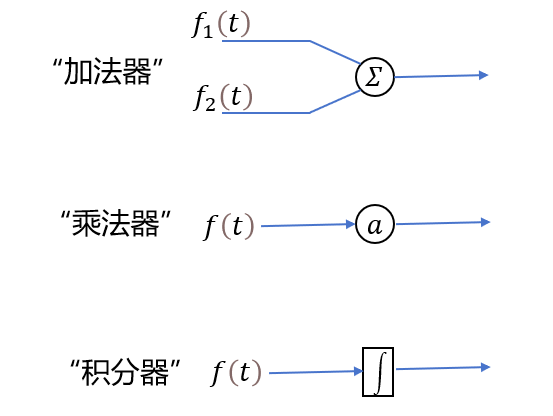
\includegraphics[scale=0.45]{6.png}
    \caption{基本框图元素}
\end{figure}
\end{document}